\documentclass[tikz,border=2pt]{standalone}
\usepackage{amsmath,amssymb}
\usepackage{tikz}
\usetikzlibrary{arrows.meta}

\begin{document}
% For n = 2 the third derivative is a 2x2x2 cube of numbers f_{ijk}; contracting it with the
% displacement h three times gives the cubic Taylor term.
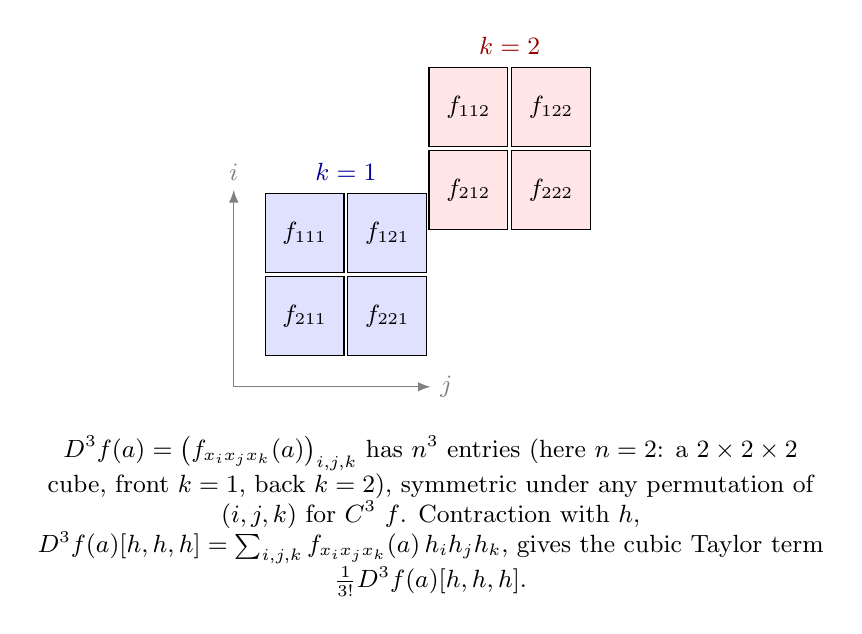
\begin{tikzpicture}[every node/.style={font=\small}, >={Latex[length=1.6mm]}]
	\begin{scope}[x={(1cm,0)}, y={(0,1cm)}, z={(1.3cm,1.0cm)}]
		% front face (k = 1)
		\foreach \i/\j/\lab in {0/1/f_{111}, 1/1/f_{121}, 0/0/f_{211}, 1/0/f_{221}} {
			\node[draw, fill=blue!12, minimum size=1cm, inner sep=0pt] at (\i*1.05,\j*1.05,0) {$\lab$};
		}
		% back face (k = 2)
		\foreach \i/\j/\lab in {0/1/f_{112}, 1/1/f_{122}, 0/0/f_{212}, 1/0/f_{222}} {
			\node[draw, fill=red!10, minimum size=1cm, inner sep=0pt] at (\i*1.05,\j*1.05,1.6) {$\lab$};
		}
		\draw[->, gray] (-0.9,-0.9,0) -- (1.6,-0.9,0) node[right] {$j$};
		\draw[->, gray] (-0.9,-0.9,0) -- (-0.9,1.6,0) node[above] {$i$};
		\node[blue!60!black, anchor=south] at (0.525,1.6,0) {$k=1$};
		\node[red!60!black, anchor=south] at (0.525,1.6,1.6) {$k=2$};
	\end{scope}
	\node[anchor=north, align=flush center, text width=10cm] at (1.6,-1.4) {$D^3f(a)=\big(f_{x_ix_jx_k}(a)\big)_{i,j,k}$ has $n^3$ entries (here $n=2$: a $2\times2\times2$ cube, front $k=1$, back $k=2$), symmetric under any permutation of $(i,j,k)$ for $C^3$ $f$. Contraction with $h$, $D^3f(a)[h,h,h]=\sum_{i,j,k}f_{x_ix_jx_k}(a)\,h_ih_jh_k$, gives the cubic Taylor term $\tfrac1{3!}D^3f(a)[h,h,h]$.};
\end{tikzpicture}
\end{document}
